\documentclass[12pt,a4paper,twoside]{report}
\usepackage[a4paper,outer=1cm,inner=3cm,top=2cm,bottom=1cm]{geometry}
\usepackage{setspace}
\usepackage{polyglossia}
\usepackage{fontspec}
\usepackage{xltxtra}
\usepackage{listings}
\usepackage{titlesec}
\usepackage{color}
\usepackage{xcolor}

\defaultfontfeatures{Scale=MatchLowercase}
\setsansfont[Mapping=tex-text]{Helvetica}
\renewcommand*{\familydefault}{\sfdefault}

\usepackage{amsmath}
\usepackage{amsfonts}

\titleformat{\section}{\normalfont\fontsize{25}{25}\bfseries\centering}{\thesection}{1em}{}
\newcommand{\sectionbreak}{\clearpage}

\title{
	Компьютерный праткикум по\\
	линейной алгебре.\\
	Расчётное задание №2\\[4em]
}
\author{Вилков Кирилл Олегович, группа 14ПИ}
\date{01.12.14}

\makeatletter
\def\Title{Расчётное задание №1}
\let\theauthor\@author
\makeatother

\usepackage{fancyhdr}
\pagestyle{fancy}
\fancyhf{}
\fancyhead[LE,RO]{\thepage}
\fancyhead[RE,LO]{\Title \qquad \theauthor}
\fancyheadoffset{0mm}
\fancyfootoffset{0mm}
\setlength{\headheight}{15pt}
\renewcommand{\headrulewidth}{1pt}
\renewcommand{\footrulewidth}{0pt}

\usepackage{tocloft}

\setcounter{tocdepth}{1}
\setcounter{secnumdepth}{0}
\renewcommand\contentsname{Содержание}
\tocloftpagestyle{fancy}

\usepackage{listings}
%\usepackage{courier}

\definecolor{dkgreen}{rgb}{0,0.6,0}
\definecolor{gray}{rgb}{0.5,0.5,0.5}
\definecolor{mauve}{rgb}{0.58,0,0.82}

\lstset{
	frame=tb,
	xleftmargin=20pt,
	language=Matlab,
	aboveskip=3mm,
	belowskip=3mm,
	showstringspaces=false,
	columns=flexible,
	basicstyle={\small\ttfamily},
	numbers=none,
	breaklines=true,
	breakatwhitespace=true
	tabsize=2
}

\newcommand{\showcode}[1]{
	%\begin{minipage}{\linewidth}
		\lstinputlisting{#1}
	%\end{minipage}
}
\newcommand{\showscreen}[1]{
\\ \includegraphics[scale=0.6]{#1} \\
}


\begin{document}

	\maketitle
	\pagestyle{fancy}
	\setcounter{page}{1}
	\tableofcontents
	\newpage

	\renewcommand*{\arraystretch}{1.5}

	\section{Задача 1.24}
\subsection{Задание:}
Решить
$
	\left|
		\begin{matrix}
			2 & x & 6 \\
			3 & 3 & 9 \\
			7 & 4 & 11
		\end{matrix}
	\right|
	= 0
$
\subsection{Решение:}
$
	3 \cdot 11 \cdot x + 2 \cdot 4 \cdot 9 + 2 \cdot 3 \cdot 11 -
	6 \cdot 3 \cdot 4 - 6 \cdot 3 \cdot 7 - 7 \cdot 9 \cdot x = 0
	\\[1ex]
	-30x - 60 = 0
	\\[1ex]
	x = -\dfrac{60}{30} = 2
$
\subsection{Проверим результат в среде Wolfram Mathematica:}
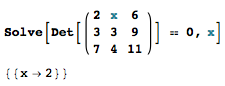
\includegraphics[scale=0.6]{task/1_24/screen.png}
\subsection{Ответ:}
Компьютерная проверка подтвердила полученный результат.

	\section{Задача 1.25}
\subsection{Задание:}
Найти матрицу обратную к
$
	A =
	\begin{pmatrix}
		2 & 4 & 0 & 1 \\
		3 & -3 & 5 & 0 \\
		-1 & 0 & 1 & 1 \\
		2 & 1 & 1 & 0 \\
	\end{pmatrix}
$
\; методом алгебраических дополненй.
\subsection{Решение:}
Найдём $ \det A $ чтобы убедиться что $ \exists A^{-1} $:
\\[1em]
$
	\det A =
	\begin{vmatrix}
		2 & 4 & 0 & 1 \\
		3 & -3 & 5 & 0 \\
		-1 & 0 & 1 & 1 \\
		2 & 1 & 1 & 0 \\
	\end{vmatrix}
	=
	\begin{vmatrix}
		3 & 4 & -1 & 0 \\
		3 & -3 & 5 & 0 \\
		-1 & 0 & 1 & 1 \\
		2 & 1 & 1 & 0 \\
	\end{vmatrix}
	=
	\begin{vmatrix}
		3 & 4 & -1 & 0 \\
		3 & -3 & 5 & 0 \\
		-1 & 0 & 1 & 1 \\
		2 & 1 & 1 & 0 \\
	\end{vmatrix}
	=
	-
	\begin{vmatrix}
		3 & 4 & -1 \\
		3 & -3 & 5 \\
		2 & 1 & 1 \\
	\end{vmatrix}
	=
	5
$
\\[1em]
$ \det A \neq 0 \Rightarrow \exists A^{-1} = \dfrac{D^T}{\det A} $
\\[1em]
$
	d_{11} =
	\begin{vmatrix}
		-3 & 5 & 0 \\
		0 & 1 & 1 \\
		1 & 1 & 0 \\
	\end{vmatrix}
	=
	\begin{vmatrix}
		-3 & 5 & 0 \\
		0 & 1 & 1 \\
		1 & 1 & 0 \\
	\end{vmatrix}
	=
	-
	\begin{vmatrix}
		-3 & 5 \\
		1 & 1 \\
	\end{vmatrix}
	= 8
\\[1em]
	d_{12} =
	\begin{vmatrix}
		3 & 5 & 0 \\
		-1 & 1 & 1 \\
		2 & 1 & 0 \\
	\end{vmatrix}
	=
	-
	\begin{vmatrix}
		3 & 5 \\
		2 & 1 \\
	\end{vmatrix}
	=
	7
\\[1em]
	d_{13} =
	\begin{vmatrix}
		3 & -3 & 0 \\
		-1 & 0 & 1 \\
		2 & 1 & 0 \\
	\end{vmatrix}
	=
	-
	\begin{vmatrix}
		3 & -3 \\
		2 & 1 \\
	\end{vmatrix}
	=
	-9
\\[1em]
	d_{14} =
	\begin{vmatrix}
		3 & -3 & 5 \\
		-1 & 0 & 1 \\
		2 & 1 & 1 \\
	\end{vmatrix}
	=
	\begin{vmatrix}
		-3 & 5 \\
		1 & 1 \\
	\end{vmatrix}
	-
	\begin{vmatrix}
		3 & -3 \\
		2 & 1 \\
	\end{vmatrix}
	=
	-8 - 9 = -17
\\[1em]
	d_{21} =
	\begin{vmatrix}
		4 & 0 & 1 \\
		0 & 1 & 1 \\
		1 & 1 & 0 \\
	\end{vmatrix}
	=
	4
	\begin{vmatrix}
		1 & 1 \\
		1 & 0
	\end{vmatrix}
	+
	\begin{vmatrix}
		0 & 1 \\
		1 & 1
	\end{vmatrix}
	= -4 - 1 = -5
\\[1em]
	d_{22} =
	\begin{vmatrix}
		2  & 0 & 1 \\
		-1 & 1 & 1 \\
		2 & 1 & 0 \\
	\end{vmatrix}
	=
	2
	\begin{vmatrix}
		1 & 1 \\
		1 & 0 \\
	\end{vmatrix}
	+
	\begin{vmatrix}
		-1 & 1 \\
		2 & 1 \\
	\end{vmatrix}
	= -2 - 3 = -5
\\[1em]
$

	\section{Задача 1.26}
\subsection{Задание:}
Решить систему линейных уравнений методом Крамера в компьютерной среде
\\[1em]
$
	\begin{cases}
		3x_1 + 2x_2 + x_3 = 5  \\
		2x_1 + 3x_2 + x_3 = 1  \\
		2x_1 + x_2 + 3x_3 = 11 \\
	\end{cases}
$
\subsection{Решение:}
Решим СЛУ в системе Wolfram Mathematica:
Найдём $ \Delta $:
\\
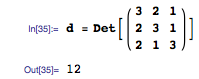
\includegraphics[scale=0.6]{task/1_26/screen1.png}
\\
Найдём $ \Delta_1, \Delta_2, \Delta_3 $:
\\
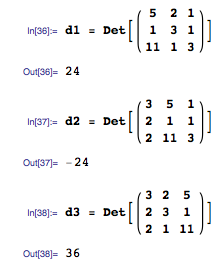
\includegraphics[scale=0.6]{task/1_26/screen2.png}
\\
Найдём корни уравнения:
\\
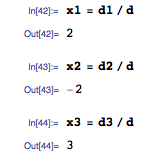
\includegraphics[scale=0.6]{task/1_26/screen3.png}
\\
\subsection{Вывод:}
Мы нашли решение системы методом Крамера: $ x_1 = 2, x_2 = -2, x_3 = 3 $.

	\section{Задача 1.27}
\subsection{Задание:}
Не вычисляя определитель
$
	\begin{vmatrix}
		2 & 1 & 7 & 8 & 1 \\
		3 & 9 & 7 & 7 & 4 \\
		6 & 5 & 3 & 4 & 3 \\
		8 & 0 & 4 & 9 & 5 \\
		7 & 2 & 9 & 1 & 9 \\
	\end{vmatrix}
$
доказать что он делится нацело на 947.
\subsection{Решение:}
По свойству определителя к любомоу столбцу можно прибавить линейную комбинацию других, и определитель не изменится.
Прибавим к последнему столбцу линейную комбинацию других:
\\
$
	\tilde a_{\bullet 5} =
	10000 \cdot a_{\bullet 1} +
	1000  \cdot a_{\bullet 2} +
	100   \cdot a_{\bullet 3} +
	10    \cdot a_{\bullet 4}
	+ a_{\bullet 5}
$
\\
Тогда определитель принимает вид:
\\[1em]
$
	\begin{vmatrix}
		2 & 1 & 7 & 8 & 21781 \\
		3 & 9 & 7 & 7 & 39774 \\
		6 & 5 & 3 & 4 & 65343 \\
		8 & 0 & 4 & 9 & 80495 \\
		7 & 2 & 9 & 1 & 72919 \\
	\end{vmatrix}
	=
	947 \cdot
	\begin{vmatrix}
		2 & 1 & 7 & 8 & 23 \\
		3 & 9 & 7 & 7 & 42 \\
		6 & 5 & 3 & 4 & 69 \\
		8 & 0 & 4 & 9 & 85 \\
		7 & 2 & 9 & 1 & 77 \\
	\end{vmatrix}
$
\\[1em]
Значит определитель делится нацело на 947
\subsection{Компьютерная проверка в среде Wolfram Mathematica:}
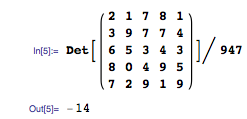
\includegraphics[scale=0.6]{task/1_27/screen1.png}
\subsection{Вывод:}
Компьютерная проверка показала что определитель действительно делится нацело на 947.

	\section{Задача 1.31}
\subsection{Задание:}
Вычислить
$
	\begin{vmatrix}
		1 & 2 & 3 & \cdots & n - 1 & n \\
		-1 & 0 & 3 & \cdots & n - 1 &  n \\
		-1 & -2 & 0 & \cdots & n - 1 & n \\
		\vdots & \vdots & \vdots & \ddots & \vdots & \vdots \\
		-1 & -2 & -3 & \cdots & -(n - 1) & 0 \\
	\end{vmatrix}
$.
\subsection{Решение:}
Вынесем общий множитель из каждого столбца определителя (вынесем из каждого столбца номер этого столбца),
тогда определитель принимает вид:
\\[1em]
$
	n! \cdot
	\begin{vmatrix}
		1 & 1 & 1 & \cdots & 1 & 1 \\
		-1 & 0 & 1 & \cdots & 1 &  1 \\
		-1 & -1 & 0 & \cdots & 1 & 1 \\
		\vdots & \vdots & \vdots & \ddots & \vdots & \vdots \\
		-1 & -1 & -1 & \cdots & -1 & 0 \\
	\end{vmatrix}
$
\\[1em]
Докажем методом мат. индукции что
$
	\begin{vmatrix}
		1 & 1 & 1 & \cdots & 1 & 1 \\
		-1 & 0 & 1 & \cdots & 1 &  1 \\
		-1 & -1 & 0 & \cdots & 1 & 1 \\
		\vdots & \vdots & \vdots & \ddots & \vdots & \vdots \\
		-1 & -1 & -1 & \cdots & -1 & 0 \\
	\end{vmatrix}
	= 1
$
\\[1em]
Проверим базу $ n = 1 $: $ |1| = 1 $
\\
Предположим что утверждение верно для $ n $, тогда докажем для $ n + 1 $:
\\[1em]
$
	\begin{vmatrix}
		1 & 1 & 1 & \cdots & 1 & 1 \\
		-1 & 0 & 1 & \cdots & 1 &  1 \\
		-1 & -1 & 0 & \cdots & 1 & 1 \\
		\vdots & \vdots & \vdots & \ddots & \vdots & \vdots \\
		-1 & -1 & -1 & \cdots & -1 & 0 \\
	\end{vmatrix}_{n + 1}
	=
	\begin{vmatrix}
		1 & 1 & 1 & \cdots & 1 & 1 \\
		-1 & 0 & 1 & \cdots & 1 &  1 \\
		-1 & -1 & 0 & \cdots & 1 & 1 \\
		\vdots & \vdots & \vdots & \ddots & \vdots & \vdots \\
		0 & 0 & 0 & \cdots & 0 & 1 \\
	\end{vmatrix}_{n + 1}
	=
	1 \cdot
	\begin{vmatrix}
		1 & 1 & 1 & \cdots & 1 & 1 \\
		-1 & 0 & 1 & \cdots & 1 &  1 \\
		-1 & -1 & 0 & \cdots & 1 & 1 \\
		\vdots & \vdots & \vdots & \ddots & \vdots & \vdots \\
		-1 & -1 & -1 & \cdots & -1 & 0 \\
	\end{vmatrix}_{n}
$
\\[1em]
Утверждение доказано.
\\[1em]
Получается что
$
	\begin{vmatrix}
		1 & 2 & 3 & \cdots & n - 1 & n \\
		-1 & 0 & 3 & \cdots & n - 1 &  n \\
		-1 & -2 & 0 & \cdots & n - 1 & n \\
		\vdots & \vdots & \vdots & \ddots & \vdots & \vdots \\
		-1 & -2 & -3 & \cdots & -(n - 1) & 0 \\
	\end{vmatrix}
	=
	n!
$
\subsection{Компьютерная проверка:}
Выполним проверку в среде Wolfram Mathematica при $ n = 8 $:
\\
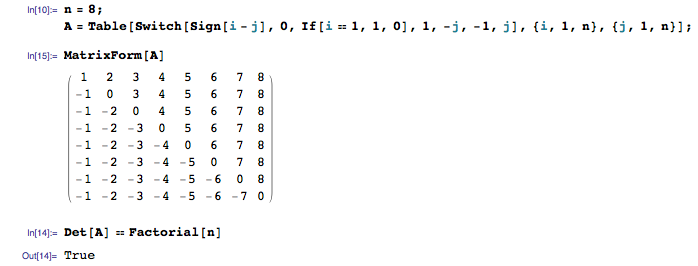
\includegraphics[scale=0.6]{task/1_31/screen1.png}
\subsection{Вывод:}
Компьютерная проверка подтвертила правильность полученной формулы.

	%\section{Задача 1.33}
\subsection{Задание:}
Вычислить:
\\[1em]
$
	\begin{vmatrix}
		0 & 1 & 1 & 1 & \cdots & 1 & 1 \\
		1 & a_1 & 0 & 0 & \cdots & 0 & 0 \\
		1 & 0 & a_2 & 0 & \cdots & 0 & 0 \\
		\vdots & \vdots & \vdots & \vdots & \ddots & \vdots & \vdots \\
		1 & 0 & 0 & 0 & \cdots & a_{n-1} & 0 \\
		1 & 0 & 0 & 0 & \cdots & 0 & a_n \\
	\end{vmatrix}
$
\subsection{Решение:}
Можно заметить что для различных $ n $ определитель такой матрицы равен
$ |A| = -\sum \limits_{i=1}^n \dfrac{1}{a_i} \prod \limits_{i=1}^n a_i $
\\
Докажем методом математической индукции:
\\
При $ n = 2 $:
\\
$
	\begin{vmatrix}
		0 & 1 & 1 \\
		1 & a_1 & 0 \\
		1 & 0 & a_2 &
	\end{vmatrix}
	= -a_1 - a_2
$
\\
Если утверждение верно при $ n $, тогда при $ n + 1 $
\\
$
\begin{vmatrix}
	0 & 1 & 1 & 1 & \cdots & 1 & 1 \\
	1 & a_1 & 0 & 0 & \cdots & 0 & 0 \\
	1 & 0 & a_2 & 0 & \cdots & 0 & 0 \\
	\vdots & \vdots & \vdots & \vdots & \ddots & \vdots & \vdots \\
	1 & 0 & 0 & 0 & \cdots & a_{n} & 0 \\
	1 & 0 & 0 & 0 & \cdots & 0 & a_{n+1} \\
\end{vmatrix}
= (-1)^{n+2} \cdot (-1)^{n+1} \cdot
\begin{vmatrix}
	0 & 1 & 1 & 1 & \cdots & 1 & 1 \\
	1 & a_1 & 0 & 0 & \cdots & 0 & 0 \\
	1 & 0 & a_2 & 0 & \cdots & 0 & 0 \\
	\vdots & \vdots & \vdots & \vdots & \ddots & \vdots & \vdots \\
	1 & 0 & 0 & 0 & \cdots & a_{n-1} & 0 \\
	1 & 0 & 0 & 0 & \cdots & 0 & a_n \\
\end{vmatrix}
- \sum \limits_{i=1}^n \dfrac{1}{a_i} \prod \limits_{i=1}^{n+1} a_i =
- \sum \limits_{i=1}^{n+1} \dfrac{1}{a_i} \prod \limits_{i=1}^{n+1} a_i
$
\subsection{Выполним компьютерную проверку в среде Wolfram Mathematica:}
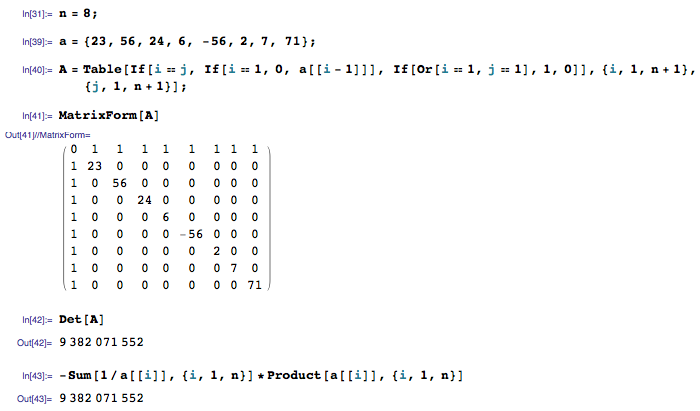
\includegraphics[scale=0.6]{task/1_33/screen.png}
\subsection{Вывод:}
Мы выполнили компьютерную проверку и убедились в верности предположения.

	\section{Задача 1.35}
\subsection{Задание:}
Вычислить $ \det A, A = \{ a_{ij} \} |, i = \overline{1,n}, j = \overline{1,n}, a_{ij} = \min (i,j) $
\subsection{Решение:}
Докажем методом мат. индукции что $ \det A = 1 $:
\\
Проверим базу индукции: $ |1| = 1 $
\\
Допустим что утверждение верно для $ n $, тогда докажем что оно будет верно для $ n + 1 $:
\\[1em]
$
	\begin{vmatrix}
		     1 &      1 & \cdots &      1 &       1 \\
		\vdots & \vdots & \ddots & \vdots &  \vdots \\
		     1 &      2 & \cdots &      n &       n \\
		     1 &      2 & \cdots &      n &   n + 1 \\
	\end{vmatrix}_{n + 1}
	=
	\begin{vmatrix}
		     1 &      1 & \cdots &      1 &       1 \\
		\vdots & \vdots & \ddots & \vdots &  \vdots \\
		     1 &      2 & \cdots &      n &       n \\
		     0 &      0 & \cdots &      0 &       1 \\
	\end{vmatrix}_{n + 1}
	=
	\begin{vmatrix}
		     1 &      1 & \cdots &      1  \\
		\vdots & \vdots & \ddots & \vdots  \\
		     1 &      2 & \cdots &      n  \\
	\end{vmatrix}_n
$
\\[1em]
В силу мат. индукции предположение доказано.
\subsection{Компьютерная проверка в среде Wolfram Mathematica:}
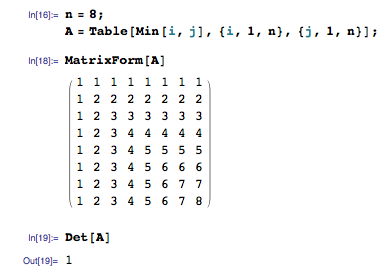
\includegraphics[scale=0.6]{task/1_35/screen1.png}
\subsection{Вывод:}
Компьютерная проверка показала что утверждение верно.

	\section{Задача 1.38}
\subsection{Задание:}
Как изменится определитель если в нём:\\
а) к каждой строке, кроме последней, прибавить последнюю строку;\\
б) из каждой строки, кроме последней, вычесть все последующие строки;\\
в) из каждой строки, кроме последней, вычесть последующую строку, а из последней вычесть бывшую первоначально первой;\\
г) повернуть его матрицу на $ 90 $ градусов вокруг центра по часовой стрелке;\\
д) первый столбец поставить на последнее место, сохранив порядок следования остальных столбцов.\\
\subsection{К каждой строке, кроме последней, прибавить последнюю строку:}
По свойству определителя если к любой строке определителя прибавить другую строку определителя, он не изменится.
Значит и в результате данного преобразования определитель не изменится.
\subsection{Из каждой строки, кроме последней, вычесть все последующие строки:}
По свойству определителя если к любой строке определителя прибавить линейную комбинацию других строк определителя, он не изменится.
Значит и в результате данного преобразования определитель не изменится.
\subsection{Из каждой строки, кроме последней, вычесть последующую строку, а из последней вычесть бывшую первоначально первой}
Пусть есть матрица $ A $ над которой мы будем производить такую операцию.
Эта операция равнозначна умножению слева матрицы $ A $ на матрицу
$
	B =
	\begin{pmatrix}
		1      & -1     & 0      & \cdots & 0      & 0      \\
		0      & 1      & -1     & \cdots & 0      & 0      \\
		\vdots & \vdots & \vdots & \ddots & \vdots & \vdots \\
		0      & 0      & 0      & \cdots & 1      & -1     \\
		-1     & 0      & 0      & \cdots & 0      & 1      \\
	\end{pmatrix}
$. По свойству определителя $ |BA| = |B| \cdot |A| $. Найдём $ |B| $ разложив его по последней строке:
\\[1em]
$
	B \in M(n)
	\\[1em]
	|B| = (-1)^{n+1} \cdot
	\begin{vmatrix}
		-1     & 0      & \cdots & 0      & 0      \\
		1      & -1     & \cdots & 0      & 0      \\
		\vdots & \vdots & \ddots & \vdots & \vdots \\
		0      & 0      & \cdots & 1      & -1     \\
	\end{vmatrix}
	+
	\begin{vmatrix}
		1      & -1     & 0      & \cdots & 0      \\
		0      & 1      & -1     & \cdots & 0      \\
		\vdots & \vdots & \vdots & \ddots & \vdots \\
		0      & 0      & 0      & \cdots & -1     \\
		0      & 0      & 0      & \cdots & 1      \\
	\end{vmatrix}
	=
	\\[1em]
	=
	(-1)^{n+1} \cdot (-1)^n + 1 = -1 + 1 = 0
$
\\[1em]
Тогда $ |BA| = 0 \cdot |A| = 0 $, в результате такого преобразования определеитель станет равен нулю.
\subsection{Повернуть его матрицу на $ 90 $ градусов вокруг центра по часовой стрелке}
Чтобы повернуть матрицу на $ 90 $ градусов транспонируем её, а потом умножим справа на матрицу
\\[1em]
$
	B =
	\begin{pmatrix}
		0 & \cdots & 0 & 1 \\
		0 & \cdots & 1 & 0 \\
		\vdots & \ddots & \vdots & \vdots \\
		1 & \cdots & 0 & 0 \\
	\end{pmatrix}
\\
	|B| = (-1)^{\left[\frac{n}{2}\right]}
$ значит изменённый определитель $ |A'| = (-1)^{\left[\frac{n}{2}\right]} \cdot |A| $
\subsection{Первый столбец поставить на последнее место, сохранив порядок следования остальных столбцов}
Для этого последовательно будем менять $ i $-ый и $ i+1 $-ый столбцы начиная с $ i = 1 $ до $ n - 1 $.
При каждой замене знак определителя будет меняться на противоположный, всего замен $ n - 1 $, значит $ |A'| = (-1)^{n-1} \cdot |A| $.

	\section{Задача 2.1}
\subsection{Задание:}
Вычислить
$
	\dfrac{(2 + 2i)^2 - (1 - i)^3}{(3 + 2i)^3 - (2 + i)^2}
$
\subsection{Решение:}
$
	\dfrac{(2 + 2i)^2 - (1 - i)^3}{(3 + 2i)^3 - (2 + i)^2}
	=
	\dfrac{8i + 2i}{-9 + 46i - 3 - 4i}
	=
	\dfrac{10i}{-12 + 42i}
	=
	\dfrac{35}{159} - \dfrac{17}{159} i
$
\subsection{Проверка в среде Wolfram Mathematica:}
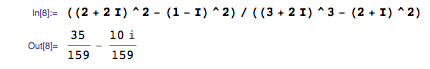
\includegraphics[scale=0.6]{task/2_01/screen1.png}
\subsection{Вывод:}
Мы вычилслили значение выражения и проверили результат в компьютерной среде.

	\section{Задача 2.2}
\subsection{Задание:}
Вычислить
$
	\dfrac{(1+i)^9}{(1-i)^9}
$
\subsection{Решение:}
$
	\dfrac{(1+i)^9}{(1-i)^9}
	=
	(\dfrac{(1+i)}{(1-i)})^9
	=
	(\dfrac{(1+i)(1+i)}{(1+i)(1-i)})^9
	=
	(\dfrac{1 - 2i - 1}{1 + 1})^9
	=
	\\[1em]
	=
	(-i)^{25}
	=
	(-i)^{24} \cdot i
	=
	(-1)^{12} \cdot i
	=
	1 \cdot i
	=
	i
$
\subsection{Компьютерная проверка в среде Wolfram Mathematica}
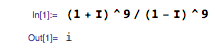
\includegraphics[scale=0.6]{task/2_02/screen1.png}
\subsection{Вывод:}
Мы правильно вычислили значение выражения.

	\section{Задача 2.3}
\subsection{Задание:}
$
	\begin{cases}
		(1 + i)x + (1 + 2i)y + (1 + 3i)z + (1 + 4i)t = 1 + 5i \\
		(3 - i)x + (4 - 2i)y + (1 + i)z + 4it = 2 - i
	\end{cases}
$
\subsection{Решение:}
Преобразуем систему:
\\[1em]
$
	\begin{cases}
		x + y + z + t = 1 \\
		3x + 4y + z = 2 \\
		ix + 2iy + 3iz + 4it = 5i \\
		-ix -2iy + iz + 4it = -i
	\end{cases}
$
\\[1em]
Разделим последние две строчки на $ i $:
\\[1em]
$
\begin{cases}
	x + y + z + t = 1 \\
	3x + 4y + z = 2 \\
	x + 2y + 3z + 4t = 5 \\
	-x -2y + z + 4t = -1
\end{cases}
$
\\[1em]
Решим систему методом Крамера:
\\[1em]
$
	\Delta =
	\begin{vmatrix}
		1 & 1 & 1 & 1 \\
		3 & 4 & 1 & 0 \\
		1 & 2 & 3 & 4 \\
		-1 & -2 & 1 & 4 \\
	\end{vmatrix} = 8
	\\[1em]
	\Delta_x =
	\begin{vmatrix}
		1 & 1 & 1 & 1 \\
		2 & 4 & 1 & 0 \\
		5 & 2 & 3 & 4 \\
		-1 & -2 & 1 & 4 \\
	\end{vmatrix} = -16
	\\[1em]
	\Delta_y =
	\begin{vmatrix}
		1 & 1 & 1 & 1 \\
		3 & 2 & 1 & 0 \\
		1 & 5 & 3 & 4 \\
		-1 & -1 & 1 & 4 \\
	\end{vmatrix} = 12
	\\[1em]
	\Delta_z =
	\begin{vmatrix}
		1 & 1 & 1 & 1 \\
		3 & 4 & 2 & 0 \\
		1 & 2 & 5 & 4 \\
		-1 & -2 & -1 & 4 \\
	\end{vmatrix} = 16
	\\[1em]
	\Delta_t =
	\begin{vmatrix}
		1 & 1 & 1 & 1 \\
		3 & 4 & 1 & 2 \\
		1 & 2 & 3 & 5 \\
		-1 & -2 & 1 & -1 \\
	\end{vmatrix} = -4
	\\[1em]
	x = \dfrac{\Delta_x}{\Delta} = -2 \\[1em]
	y = \dfrac{\Delta_y}{\Delta} = \dfrac{3}{2} \\[1em]
	z = \dfrac{\Delta_z}{\Delta} = 2 \\[1em]
	t = \dfrac{\Delta_t}{\Delta} = - \dfrac{1}{2} \\[1em]
$
\subsection{Выполним компьютерную проверку в среде Wolfram Mathematica:}
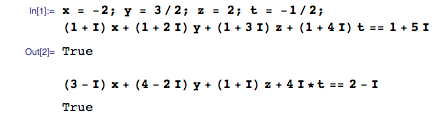
\includegraphics[scale=0.6]{task/2_03/screen1.png}
\subsection{Вывод:}
Мы верно нашли решение системы.

	\section{Задача 2.4}
\subsection{Задание:}

	\section{Задача 2.7}
\subsection{Задание:}
При каких условиях модуль суммы двух комплексных чисел равен разности модулей слагаемых?
\subsection{Решение:}
$
	z_1 = x_1 + i y_1\\
	z_2 = x_2 + i y_2\\
$
Модуль суммы $ z_1 $ и $ z_2 $ это длинна вектора, составленного как векторная сумма $ z_1 $ и $ z_2 $.\\
Таким образом модуль суммы двух комплексных чисел будет равен разности модулей слагаемых когда векторы,
соответствующие $ z_1 $ и $ z_2 $ на плоскости комплексных чисел будут противоположно направленными, то есть
должно выполняться условие:
\\[1em]
$
	\dfrac{x_1}{x_2} = \dfrac{y_1}{y_2} < 0
$
\subsection{Компьютерная проверка в среде Wolfram Mathematica}
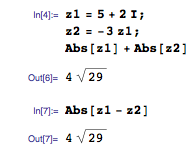
\includegraphics[scale=0.6]{task/2_07/screen1.png}
\subsection{Вывод:}
Мы нашли условие при котором модуль суммы двух комплексных чисел равен разности модулей слагаемых.

	\section{Задача 2.8}
\subsection{Задание:}
Доказать, что если в результате конечного числа рациональных операций (сложение, умножение, вычитание, деление)
выполненых над комплексными числами $ z_1, \dots, z_n $ получается комплексное число $ u $, то в результате выполнения тех же
операций над $ \overline{z_1}, \dots, \overline{z_n} $ получается $ \overline{u} $.
\subsection{Доказательство:}
Пусть $ u_j $ - результат выполнения данных операций с числами $ z_1, \dots, z_j $,
тогда $ u_j = u_{j-1} \; \circ \; z_j $.
\\
Получается что $ u_n = u, \; \overline{u_n} = \overline{u} $.
\\
Докажем что $ \overline{u_j} $ - результат выполнения данных операций с $ \overline{z_1}, \dots, \overline{z_j} $
для каждой из четырёх операций:
\subsection{Сложение:}
$
	\overline{u_j}
	=
	\operatorname{Re} \overline{u_j} + i \operatorname{Im} \overline{u_j}
	=
	\operatorname{Re} u_j - i \operatorname{Im} u_j
	=
	\operatorname{Re} u_{j-1} + \operatorname{Re} z_j - i(\operatorname{Im} u_(j-1) + \operatorname{Im} z_j)
	=
	(\operatorname{Re} u_{j-1} - i\operatorname{Im} u_{j-1}) + (\operatorname{Re} z_j - i\operatorname{Im} z_j)
	=
	\overline{u_{j-1}} + \overline{z_j}
$
\subsection{Вычитание:}
$
	\overline{u_j}
	=
	\operatorname{Re} \overline{u_j} + i \operatorname{Im} \overline{u_j}
	=
	\operatorname{Re} u_j - i \operatorname{Im} u_j
	=
	\operatorname{Re} u_{j-1} - \operatorname{Re} z_j - i(\operatorname{Im} u_(j-1) - \operatorname{Im} z_j)
	=
	(\operatorname{Re} u_{j-1} - i\operatorname{Im} u_{j-1}) - (\operatorname{Re} z_j - i\operatorname{Im} z_j)
	=
	\overline{u_{j-1}} - \overline{z_j}
$
\subsection{Умножение:}
$
	\overline{u_j}
	=
	\operatorname{Re} \overline{u_j} + i \operatorname{Im} \overline{u_j}
	=
	\operatorname{Re} u_j - i \operatorname{Im} u_j
	=
	\operatorname{Re} u_{j-1} \cdot \operatorname{Re} z_j - i(\operatorname{Im} u_{j-1} \cdot \operatorname{Im} z_j)
	=
	\operatorname{Re} u_{j-1} \cdot \operatorname{Re} z_j +
	i(\operatorname{Im} \overline{u_{j-1}} \cdot \operatorname{Im} \overline{z_j})
	=
	\overline{u_{j-1}} \cdot \overline{z_j}
$
\subsection{Деление:}
$
	\overline{u_j}
	=
	\operatorname{Re} \overline{u_j} + i \operatorname{Im} \overline{u_j}
	=
	\operatorname{Re} u_j - i \operatorname{Im} u_j
	=
	\overline{u_{j-1}} / \overline{z_j}
$
\\[2em]
Таким образом в результате тех же операций над $ \overline{z_1}, \dots, \overline{z_n} $ получается $ \overline{u} $.
\subsection{Компьютерная проверка в среде Wolfram Mathematica:}
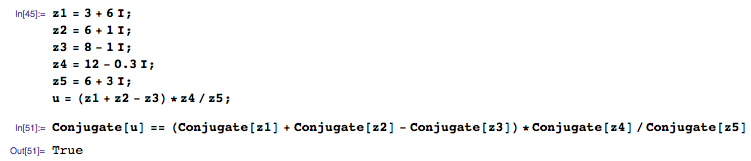
\includegraphics[scale=0.6]{task/2_08/screen1.png}
\\
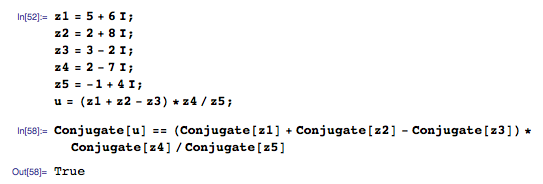
\includegraphics[scale=0.6]{task/2_08/screen2.png}
\subsection{Вывод:}
Утверждение доказано.

	\section{Задача 2.9}
\subsection{Задание:}
Доказать что всякое комплексное $ z \neq -1, |z| = 1 $ представимо в виде $ z = \dfrac{1+it}{1-it}, t \in \mathbb{R} $.
\subsection{Решение:}
$
	\dfrac{1+it}{1-it}
	=
	\dfrac{\sqrt{1+t^2}e^{i\phi}}{\sqrt{1+t^2}e^{-i\phi}}
	=
	e^{2i\phi}
$, где $ \phi = \operatorname{Arg} (1 + it) $
\\
Так как $ |z| = 1 $, $ z $ можно представить как $ e^{i\theta} $, приравняем: $ i\theta = 2i\phi $.
\\
Значит любое комплексное число $ z \neq -1, |z| = 1 $ представимо в виде $ z = \dfrac{1+it}{1-it}, t \in \mathbb{R} $.
\subsection{Выполним проверку в компьютерной среде Wolfram Mathematica:}
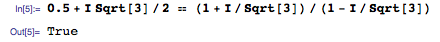
\includegraphics[scale=0.6]{task/2_09/screen.png}
\subsection{Вывод:}
Утверждение доказано и прошло проверку в компьютерной среде.

	\section{Задача 2.10}
\subsection{Задание:}
Визуализировать геометрические места точек комплексной плоскости.
\subsection{Решение:}
a) $ |z| = 1 $
\\
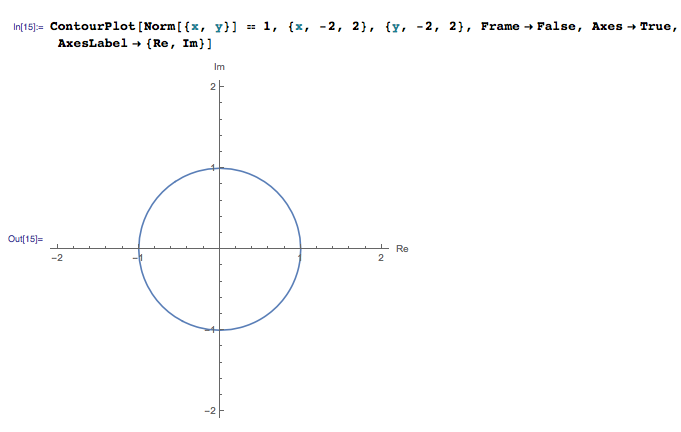
\includegraphics[scale=0.6]{task/2_10/screen1.png}
\\
б) $ \operatorname{Arg} z = \frac{1}{3}\pi $
\\
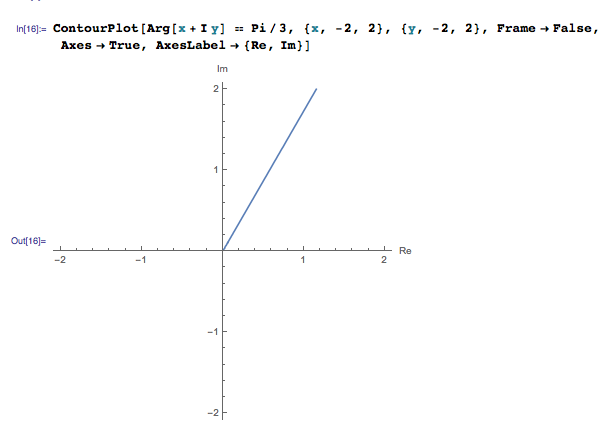
\includegraphics[scale=0.6]{task/2_10/screen2.png}
\\
в) $ |z - 1 - 2i| < 2 $
\\
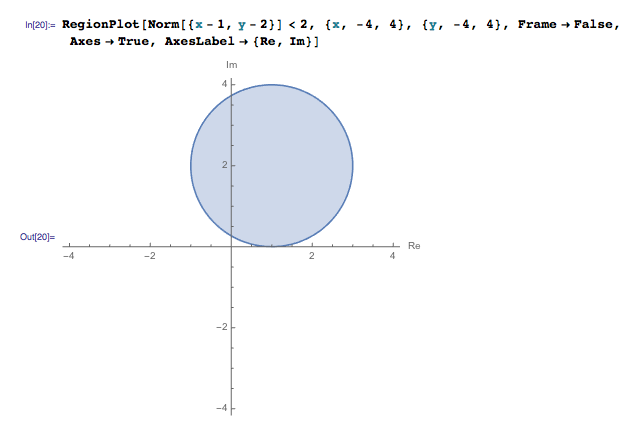
\includegraphics[scale=0.6]{task/2_10/screen3.png}
\\
г) $ |z + 3i| \geq 3 $
\\
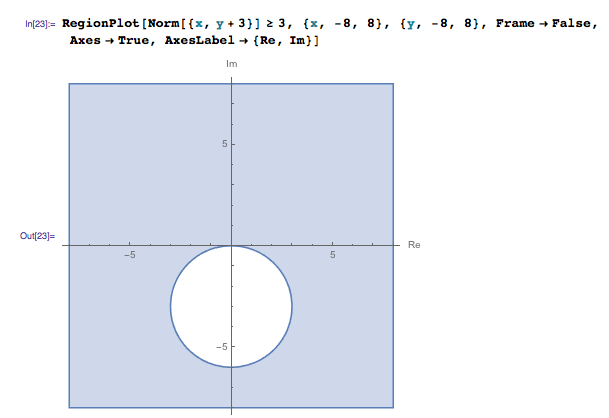
\includegraphics[scale=0.6]{task/2_10/screen4.png}
\\
д)
$
	\begin{cases}
		\operatorname{Re} z > -1
		\operatorname{Im} \leq 2
	\end{cases}
$
\\
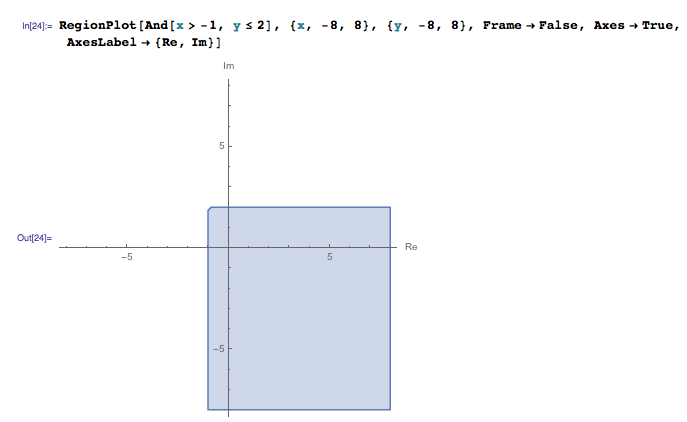
\includegraphics[scale=0.6]{task/2_10/screen5.png}
\\
е)
$ |z+i|=|z-i| $
\\
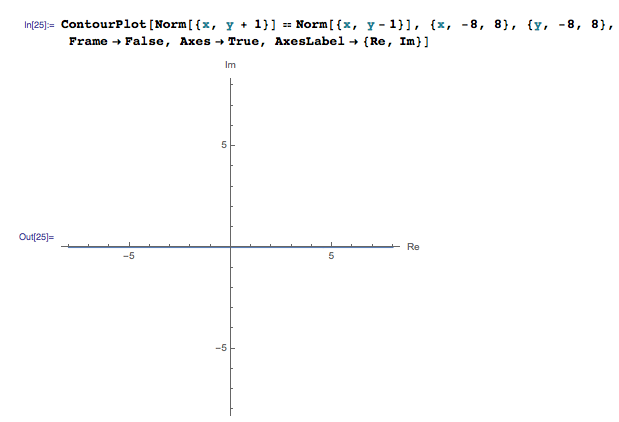
\includegraphics[scale=0.6]{task/2_10/screen6.png}
\\
ж)
$ |\pi - \operatorname{Arg} z| < \dfrac{\pi}{4}, \operatorname{Arg}z \in [0,2\pi) $
\\
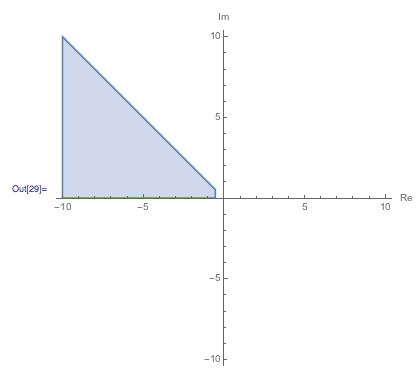
\includegraphics[scale=0.6]{task/2_10/screen7.png}
\\
з)
$
	\begin{cases}
		|z + i| < 1 \\
		-\dfrac{3\pi}{4} \leq \operatorname{Arg} z \leq -\dfrac{pi}{4}
	\end{cases}, \;
	\operatorname{Arg} z \in [-\pi,\pi)
$
\\
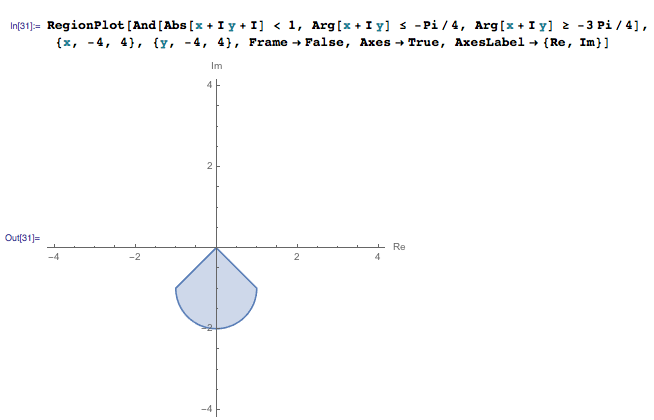
\includegraphics[scale=0.6]{task/2_10/screen8.png}
\\


\end{document}
